\documentclass[12pt]{standalone}

\usepackage{tikz}

\usetikzlibrary{positioning}
\usetikzlibrary{shapes.geometric}

\begin{document}
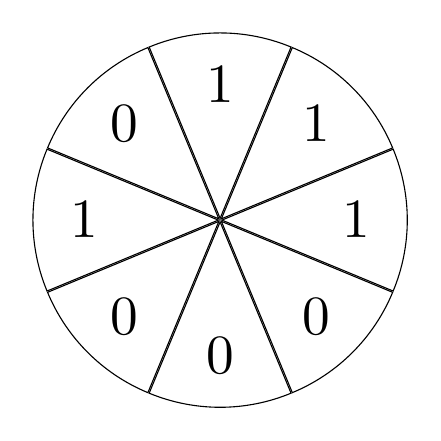
\begin{tikzpicture}[every node/.style={draw,
    circular sector,
    shape border uses incircle,
    circular sector angle=45,
    scale=2
    }]
    \begin{scope}[node distance=-20.8pt]
        % A few hacks are used to make the thing look like a circle
        \node [circle,minimum size=20pt,draw=none] (C) {};
        \node [left=of C] {1};
        \node [below left=of C,shape border rotate=45] {0};
        \node [below=of C,shape border rotate=90] {0};
        \node [below right=of C,shape border rotate=135] {0};
        \node [right=of C,shape border rotate=-180] {1};
        \node [above right=of C,shape border rotate=225] {1};
        \node [above=of C,shape border rotate=270] {1};
        \node [above left=of C,shape border rotate=315] {0};
    \end{scope}
\end{tikzpicture}
\end{document}
